\documentclass[12pt]{article}
\usepackage[UTF8]{ctex}
\usepackage{amsmath}
\usepackage{indentfirst}
\usepackage{amsmath}
\newtheorem{theorem}{Theorem}
\newtheorem{lemma}{Lemma}
\newtheorem{proof}{Proof}[section]
\usepackage{graphicx}
\setlength{\parindent}{2em}
\title{IOI2020 中国国家集训队第一阶段作业\\解题报告}
\author{成都市第七中学\ 党星宇}
\date{2019.10}
\usepackage{fancyhdr}
\pagestyle{fancy}
\lhead{\small \leftmark}
\chead{}
\rhead{\small{成都市第七中学\ 党星宇}}
\lfoot{}
\cfoot{}
\rfoot{\thepage}
\renewcommand{\headrulewidth}{0.4pt}
\renewcommand{\footrulewidth}{0.4pt}

\begin{document}
\maketitle

\newpage

\section{Coloring Balls}
\subsection{试题来源}
AtCoder Regular Contest 089 F
\subsection{题目大意}
最开始有$N$个白球排成一排。有$K$次操作,每次给出红色或蓝色两种颜色中的一种,你可以选择任意一个区间将这个区间的球成这种染色。但是不能直接将白球染成蓝色。问$K$次操作完成后有多少种可能的不同球的序列。

答案对$10^9+7$取模。
\subsection{数据范围}
$N,K\le 70$
\subsection{时空限制}
时间限制:$4$秒

空间限制:$256$MB
\subsection{解题过程}
我们先考虑一个暴力做法:$3^N$枚举所有可能的颜色状态,依次判断每一种是否合法。

但是其实我们不需要枚举所有$3^N$的可能状态,因为其中有很多是等价的。

为了表示一个颜色序列,我们用$R,B,W$分别表示红色球、蓝色球和白色球。

我们以'WRRBRBBWWRRRRWRBBWWRRBBRR'为例。

首先,按照白色将原序列分成若干段:\{'RRBRBB', 'RRRR', 'RBB', 'RRBBRR'\}。

其次,我们将相同颜色的一段缩在一起:\{'RBRB', 'R', 'RB', 'RBR'\}。

然后,我们将给每一段按照'B'的个数标号:

Group 1:'R'

Group 2:'B', 'RB', 'BR', 'RBR'

Group 3:'BRB', 'RBRB', 'BRBR', 'RBRBR'

Group 4:'BRBRB', 'RBRBRB', 'BRBRBR', 'RBRBRBR'

$\cdots$

考虑除了第一次和第二次操作只能分别为$r,b$之外,其余非平凡情况中,任意一次$r$或者$b$的操作都可以增加一个$B$。具体的,每一组的操作序列如下。

Group 1:'r'

Group 2:'rb'

Group 3:'rb?'

Group 4:'rb??'

Group 5:'rb???'

$\cdots$

我们用一个数字序列$f$表示一组颜色的等价类。由于各段显然是独立的,我们可以以任意顺序排列$f$中的元素。例如例子中的$f$=['3', '2', '2', '1']。假设$g(N)$表示$N$的拆分数,总的状态数个数是$O(g(N)\times N)$的,对于$N\le 70$,至多为$418662$。

下面我们考虑如何检验一个颜色等价类是否合法,相当于是对于颜色序列中的每一段分配一个操作子序列符合他的Group的要求,显然,我们考虑贪心地分配:
\begin{itemize}
  \item 首先将$f$按从大到小排序
  \item 对于每个$k$,将$S$中的第$k$个'r'(它的位置记为$r_k$)分配给$f[k]$
  \item 对于每一个$f[k]=x$,(我们从左到右依次考虑每一个$f[i]$),如果$x\ge 2$,那么将$r_k$右边最靠左的$b$(它的位置记为$b_k$)分配给它。
  \item 对于每一个$f[k]=x$,如果$x\ge 3$,就把$b_k$右边未被使用的最近$x-2$个操作分配给它。
\end{itemize}

这个贪心的复杂度足以通过本题。

我们考虑对于一个等价类集合$f$如何统计它的方案数。

首先考虑将每一段作为整体排列的方案数,显然是$\frac{|f|!}{\prod_{i=1}^{n}cnt_i!}$,其中$cnt_i$表示$f_k=i$的$k$的个数。

然后我们考虑原序列被划分成了多少个颜色相同的连续段。

容易发现除了Group 1只能是一段$R$之外,其余的Group x$(x \ge 2)$都可以是$(R)B...B(R)$(长度为$2x-1$),左右两个$R$可以为空的形式。而为白色的段最左边和最右边可以为空,而在两个Group之间的白色段不能为空。故用挡板法很容易得到这部分的方案数为
$$
\binom{N + 1 + \sum_{v\in f, v\ge 2} 2}{\sum_{v\in f} v\times 2}
$$

\subsection{总结}
本题是一道经典的atcoder风格计数题目,难度较大,主要考察了选手对于计数问题模型的分析能力。

本题需要从状态入手,首先将序列分成若干段,其中每段独立,然后将相同颜色部分的合并。通过分析操作的性质,将状态按照$'B'$的段数进行分类,将等价的状态合并。然后发现本质不同的状态数很少,于是可以逐一判断其合法性。在合法性判断时,需要运用简单的贪心技巧。在代码实现上也较为简单,是一道优秀的计数题目。

\newpage

\section{Spiders Evil Plan}
\subsection{试题来源}
ZeptoLab Code Rush 2015  G
\subsection{题目大意}
有一棵$n$个点的树,边有边权$l_i$。有$q$次询问,每次给$x,y$,查询由任意$y$条链的并组成的所有包含点$x$联通块中边权和的最大值(强制在线)。

\subsection{数据范围}
$1\le n, q\le 10^5, 1\le l_i \le 1000$
\subsection{时空限制}
时间限制:$1$秒

空间限制:$256$MB
\subsection{解题过程}
显然选择的所有链的两端一定为叶子,并且选择的链一定是一个连通块(如果不是可以调整使得答案不会变小,如下图)
\begin{figure}[h] %figure环境,h默认参数是可以浮动,不是固定在当前位置。如果要不浮动,你就可以使用大写float宏包的H参数,固定图片在当前位置,禁止浮动。
    \centering %使图片居中显示
    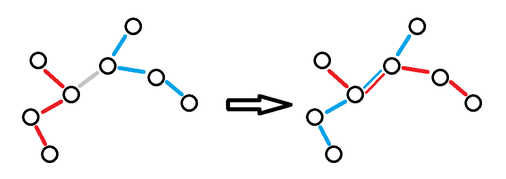
\includegraphics[width=0.5\textwidth]{p1.png} %中括号中的参数是设置图片充满文档的大小,你也可以使用小数来缩小图片的尺寸。
    \label{p1} %这是添加标签,方便在文章中引用图片。
\end{figure}%figure环境

更进一步的,我们可以得到下面这个结论:

\begin{theorem}
  对于一个树,如果它有$2k$个叶子,那么它就能被$k$条路径完全覆盖。
\end{theorem}

结论的正确性也非常显然。即如果有一条边没有被覆盖,可以通过调整两条路径得到。
\begin{figure}[h]
  \centering
  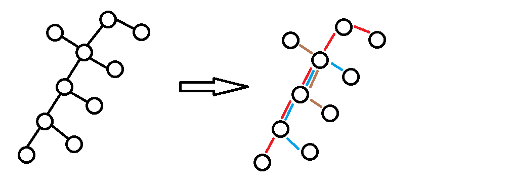
\includegraphics[width=0.5\textwidth]{p2.png}
  \label{p2}
\end{figure}

于是询问$(x,y)$可以理解为:选择$2y$个叶子,使得连通块包含$x$并且边权和最大。

我们可以考虑以$x$为根,现在的问题是如何选择叶子。

显而易见的是,如果一个节点$x$的子树中有一个叶子$u$被选择了,那么$x$所在长链包含的叶子一定也被选择了。

于是对于每一个叶子的贡献,我们单独考虑它们的贡献,贡献为它到它长链顶的距离,也就是说我们考虑依次加入长链。

于是我们按照贡献排序,依次选择即可。

但是每次都重新以$x$为根复杂度太高。我们考虑经过$x$的最长路径一定经过直径的其中一端,于是我们以直径两端分别为根做两边。

现在问题是如果$x$不被我们选择的前$2y-1$大的叶子包含怎么办?

有两种情况:一种是将贡献最小的长链去掉并加入$x$所在长链,另一种是找到离$x$最近的长链将下半部分替换成$x$所在长链,如下图(黄色是$x$,绿色是之前选的方案,红色是调整后选择的方案)。

\begin{figure}[h]
  \centering
  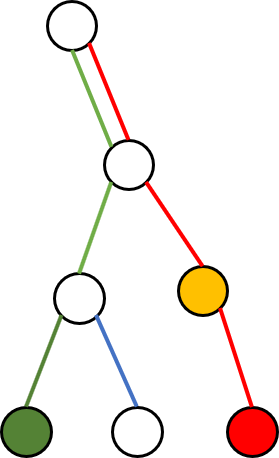
\includegraphics[width=0.1\textwidth]{p7.png}
  \label{p3}
\end{figure}

然后用倍增查找替换位置即可。

复杂度$O((n+q)\log n)$

\subsection{总结}
本题难度中等,考察选手对于树的常用性质的理解,需要选手从多方面入手分析问题,并对链并一类的问题较为熟悉才能解决。

在本题中,多次运用了调整的思想,例如考虑将两条路径的端点互换以及考虑当前方案不包含$x$时调整方案,将复杂的情况用通用的方式整合考虑。同时,将每个叶子的贡献单独考虑,并最后发现就是其所在长链的贡献也是本题的关键以及亮点。除了这些以外,本题对于一些小技巧的考察也很全面。如树上到一个点的最长路径必定经过直径一端,于是可以选择以直径一端为根。并且代码难度不大。是一道不可多得的树上好题。

\newpage

\section{Limak and Shooting Points}

\subsection{试题来源}
Codeforces Round 363 (Div. 1)

\subsection{题目大意}

平面上有$n$个怪物和$k$个射击地点,可以按照任意顺序选择每个射击地点至多一次,每个地点可以选择任意一个方向射一支箭,每次会击中这个方向上$\textbf{第一个}$怪物,射击完后箭和怪物都会消失,问有哪些怪物可能会被射击到。

\subsection{数据范围}
$1\le k\le 7,1\le n\le 1000$。

坐标在$[-10^9,10^9]$之间。

\subsection{时空限制}
时间限制:$3s$

空间限制:$256$MB

\subsection{解题过程}
我们枚举每个怪物考虑判断他是否可能被射击到。

假设在点$u$射击时,会挡住怪物$x$的怪物集合为$B_{u,x}$,这个可以事先$O(n^2k)$地用叉积和点积判断预处理所有的$B_{u,x}$。

在考虑怪物$x$是否可能被射击到时,发现$k$的范围很小,容易想到$k!$枚举所有可能的射击顺序,假设最后一次射中$x$。设枚举最后一次的射击点为$u$,那么$x$被射中的充要条件是$B_{u, x}$中的所有怪物在此之前都被射击到了。由于我们枚举所有的可能射击顺序,所以按照什么顺序分配给$B_{u,x}$中的元素是无关紧要的。同时,由于至多击中$k$怪物,所以我们每次检验时,每次访问的怪物个数至多为$k$个,于是我们每次暴力搜索所有$B_{u,x}$的元素判断是否合法,当当前处理的怪物个数$>k$时终止即可。这样的时间复杂度为$O(k!nk)$。但是如果我们不先$k!$枚举射击顺序,而是在搜索的时候同时枚举,可以将复杂度降到$O(k!n)$

故总复杂度为$O(n^2k+k!n)$,可以通过本题。

\subsection{总结}
本题难度较低,代码实现也很简单。考察了选手对于基础的计算几何能力以及按照顺序枚举判断依次考虑每一个元素的方法,是一道基础的计算几何题目。

\end{document} 